\documentclass[border=10pt]{standalone}
% Shared preamble for the README figures. Build with `docs/figures/build.sh`.
\usepackage[T1]{fontenc}
\usepackage{libertinus}
\setmonofont{Inconsolatazi4-Regular.otf}[Scale=0.86,BoldFont=Inconsolatazi4-Bold.otf]
\usepackage{amsmath}
\usepackage{tikz}
\usepackage{pgfplots}
\pgfplotsset{compat=1.18}
\usetikzlibrary{arrows.meta,positioning,calc,fit,backgrounds,decorations.pathreplacing,shapes.geometric,patterns}

\definecolor{ink}{gray}{0.11}
\definecolor{mute}{gray}{0.40}
\definecolor{faint}{gray}{0.62}
\definecolor{rule}{gray}{0.80}
\definecolor{fill}{gray}{0.955}
\definecolor{neg}{RGB}{164,38,44}
\definecolor{negfill}{RGB}{247,229,228}
\pagecolor{white}
\color{ink}

\tikzset{
  >={Stealth[length=5pt,width=4pt]},
  every picture/.style={line width=0.55pt, draw=ink},
  panel/.style={draw=rule, line width=0.6pt, fill=white},
  box/.style={draw=ink, fill=white, inner sep=3pt, font=\footnotesize},
  soft/.style={draw=rule, fill=fill, inner sep=3pt, font=\footnotesize},
  lab/.style={font=\footnotesize\color{mute}, inner sep=0pt},
  flow/.style={->, draw=ink, line width=0.7pt},
  code/.style={draw=rule, fill=fill, align=left, inner sep=4pt, font=\ttfamily\scriptsize, execute at begin node={\hyphenpenalty=10000\relax\exhyphenpenalty=10000\relax}},
}
\newcommand{\plabel}[2]{\textbf{(#1)}\,\textsc{#2}}

\usepgfplotslibrary{groupplots}
% Data: work/trail-ns/eval-gaia-judge-v2.json, eval-gaia-checks-only.json,
% eval-swe-judge.json, eval-swe-checks-only.json; tau2 from
% docs/next-state-verifier.md (run turn-judge-d450cf34d97b27a2).
\begin{document}
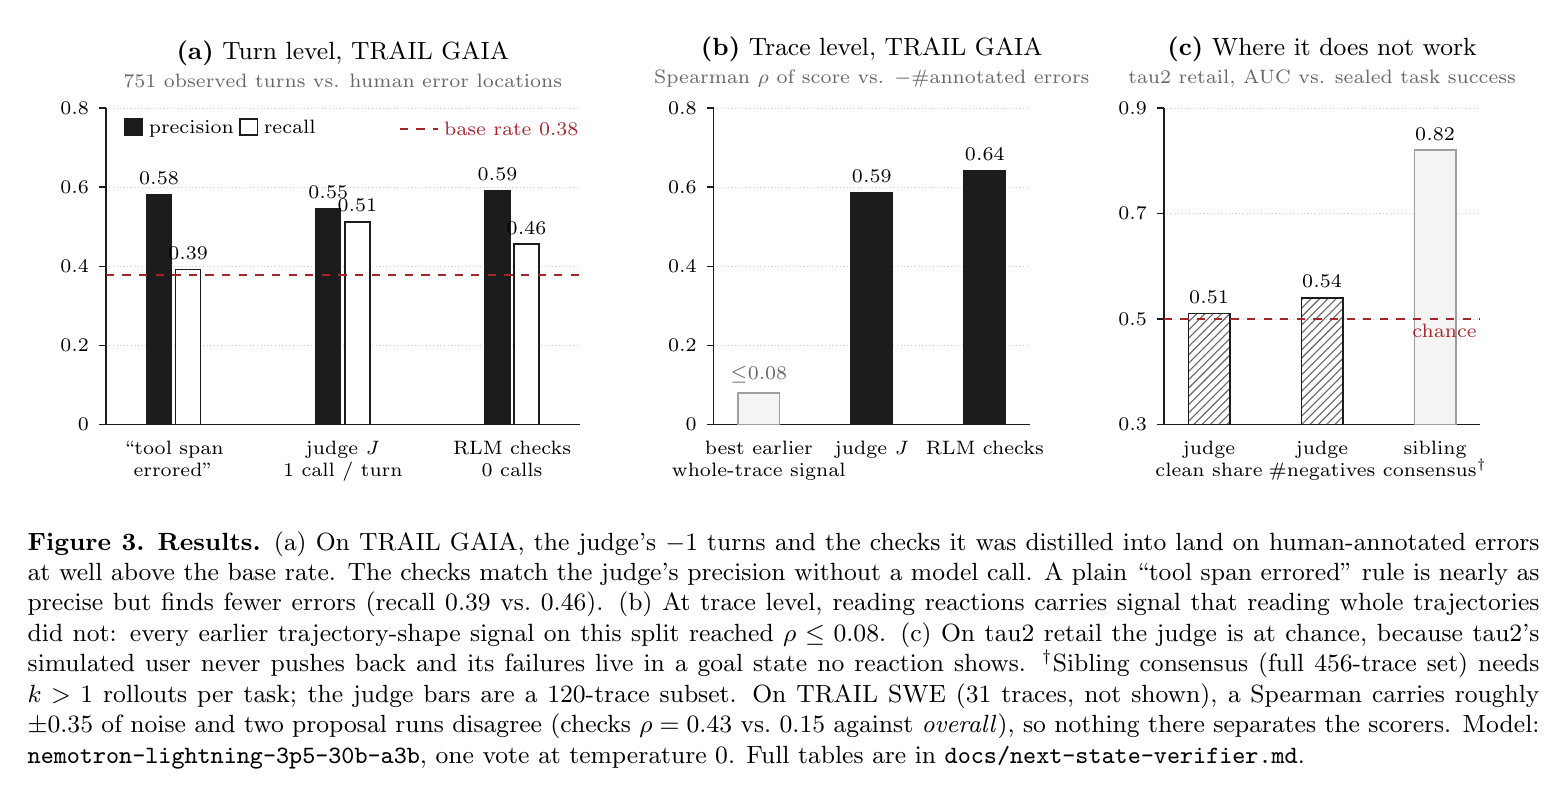
\begin{tikzpicture}
\pgfplotsset{
  every axis/.style={
    axis lines*=left, axis line style={draw=ink, line width=0.5pt},
    tick style={draw=ink, line width=0.5pt}, tick align=outside,
    major tick length=2.5pt,
    ticklabel style={font=\scriptsize},
    label style={font=\footnotesize},
    title style={font=\small, align=center, yshift=-2pt},
    ymajorgrids, grid style={draw=rule, line width=0.3pt, densely dotted},
    enlarge x limits=0.2,
    xtick style={draw=none},
    nodes near coords style={font=\scriptsize},
    legend style={font=\scriptsize, draw=none, fill=none},
  },
}
\begin{groupplot}[group style={group size=3 by 1, horizontal sep=1.7cm}, height=5.6cm]

% (a) turn-level P / R, TRAIL GAIA
\nextgroupplot[
  width=7.6cm,
  title={\textbf{(a)} Turn level, TRAIL GAIA\\[-1pt]\scriptsize\color{mute}751 observed turns vs. human error locations},
  ybar=1.5pt, bar width=9pt,
  ymin=0, ymax=0.8, ytick={0,0.2,0.4,0.6,0.8},
  symbolic x coords={tool,judge,checks},
  xtick=data,
  xticklabels={{``tool span\\errored''},{judge $J$\\1 call / turn},{RLM checks\\0 calls}},
  xticklabel style={align=center, font=\scriptsize},
  nodes near coords, nodes near coords align={vertical},
  every node near coord/.append style={/pgf/number format/.cd, fixed, fixed zerofill, precision=2},
  legend columns=2, legend style={at={(0.02,1.0)}, anchor=north west},
  legend image code/.code={\draw[#1] (0cm,-0.08cm) rectangle (0.22cm,0.12cm);},
]
\addplot[fill=ink, draw=ink] coordinates {(tool,0.581) (judge,0.545) (checks,0.592)};
\addplot[fill=white, draw=ink] coordinates {(tool,0.392) (judge,0.512) (checks,0.456)};
\legend{precision, recall}
\draw[neg, dashed, line width=0.7pt] ({rel axis cs:0,0} |- {axis cs:tool,0.377}) -- ({rel axis cs:1,0} |- {axis cs:tool,0.377});
\draw[neg, dashed, line width=0.7pt] (rel axis cs:0.62,0.935) -- (rel axis cs:0.70,0.935) node[right, font=\scriptsize, text=neg, inner sep=2pt] {base rate 0.38};

% (b) trace-level Spearman, TRAIL GAIA
\nextgroupplot[
  width=5.6cm,
  title={\textbf{(b)} Trace level, TRAIL GAIA\\[-1pt]\scriptsize\color{mute}Spearman $\rho$ of score vs. $-\#$annotated errors},
  ybar, bar width=15pt,
  ymin=0, ymax=0.8, ytick={0,0.2,0.4,0.6,0.8},
  symbolic x coords={prior,judge,checks},
  xtick={prior,judge,checks},
  xticklabels={{best earlier\\whole-trace signal},{judge $J$},{RLM checks}},
  xticklabel style={align=center, font=\scriptsize},
  nodes near coords, nodes near coords align={vertical},
  every node near coord/.append style={/pgf/number format/.cd, fixed, fixed zerofill, precision=2},
]
\addplot[fill=ink, draw=ink, bar shift=0pt] coordinates {(judge,0.587) (checks,0.642)};
\addplot[fill=fill, draw=faint, bar shift=0pt, nodes near coords={}] coordinates {(prior,0.08)};
\node[font=\scriptsize, text=mute, anchor=south] at (axis cs:prior,0.08) [yshift=0pt] {$\le$0.08};

% (c) where it does not work
\nextgroupplot[
  width=5.6cm,
  title={\textbf{(c)} Where it does not work\\[-1pt]\scriptsize\color{mute}tau2 retail, AUC vs. sealed task success},
  ybar, bar width=15pt,
  ymin=0.3, ymax=0.9, ytick={0.3,0.5,0.7,0.9},
  symbolic x coords={jc,jn,sib},
  xtick={jc,jn,sib},
  xticklabels={{judge\\clean share},{judge\\\#negatives},{sibling\\consensus$^{\dagger}$}},
  xticklabel style={align=center, font=\scriptsize},
  nodes near coords, nodes near coords align={vertical},
  every node near coord/.append style={/pgf/number format/.cd, fixed, fixed zerofill, precision=2},
]
\addplot[fill=white, draw=ink, pattern=north east lines, pattern color=mute, bar shift=0pt] coordinates {(jc,0.51) (jn,0.54)};
\addplot[fill=fill, draw=faint, bar shift=0pt] coordinates {(sib,0.82)};
\draw[neg, dashed, line width=0.7pt] ({rel axis cs:0,0} |- {axis cs:jc,0.5}) -- ({rel axis cs:1,0} |- {axis cs:jc,0.5});
\node[anchor=north east, font=\scriptsize, text=neg, inner sep=1pt] at (rel axis cs:1,0.33) {chance};
\end{groupplot}

\node[anchor=north west, text width=19.2cm, align=justify, font=\small, inner sep=0] at ($(group c1r1.south west)+(-1.0,-1.35)$) {%
\textbf{Figure 3.} \textbf{Results.} (a) On TRAIL GAIA, the judge's $-1$ turns and the checks it was distilled into land on human-annotated errors at well above the base rate. The checks match the judge's precision without a model call. A plain ``tool span errored'' rule is nearly as precise but finds fewer errors (recall 0.39 vs.\ 0.46). (b) At trace level, reading reactions carries signal that reading whole trajectories did not: every earlier trajectory-shape signal on this split reached $\rho\le0.08$. (c) On tau2 retail the judge is at chance, because tau2's simulated user never pushes back and its failures live in a goal state no reaction shows. $^{\dagger}$Sibling consensus (full 456-trace set) needs $k>1$ rollouts per task; the judge bars are a 120-trace subset. On TRAIL SWE (31 traces, not shown), a Spearman carries roughly $\pm0.35$ of noise and two proposal runs disagree (checks $\rho=0.43$ vs.\ $0.15$ against \emph{overall}), so nothing there separates the scorers. Model: \texttt{nemotron-lightning-3p5-30b-a3b}, one vote at temperature 0. Full tables are in \texttt{docs/next-state-verifier.md}.};
\end{tikzpicture}
\end{document}
